\documentclass[12pt]{article}
\usepackage{graphicx}
\graphicspath{ {./images/} }
\usepackage[margin=1in]{geometry} 
\usepackage{amsmath,amsthm,amssymb,amsfonts}
 
\newcommand{\N}{\mathbb{N}}
\newcommand{\Z}{\mathbb{Z}}
 
\newenvironment{problem}[2][Problem]{\begin{trivlist}
\item[\hskip \labelsep {\bfseries #1}\hskip \labelsep {\bfseries #2.}]}{\end{trivlist}}
 
\begin{document}

 
\title{Homework 3 - CS2300}
\author{Andrew Henningsen and Evan Wilcox}
\maketitle

\begin{enumerate}
    \item Convert the ER diagram into relational schemas.\\
        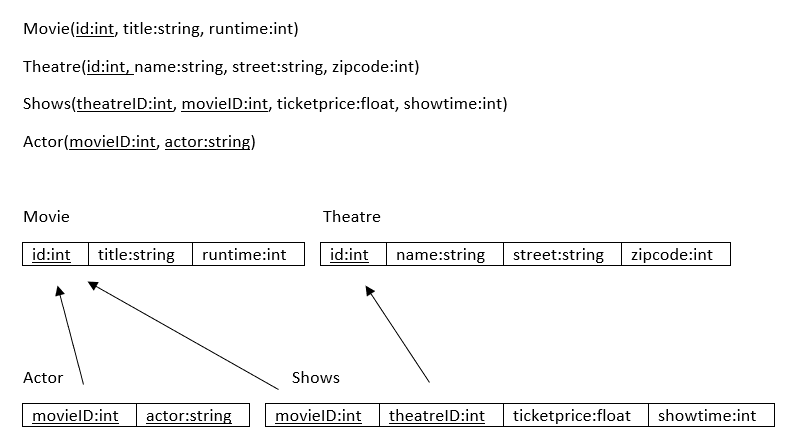
\includegraphics[scale=.9]{1}
    \item $ActorsWMid \leftarrow Actor \bowtie_{Actor.id = STARS_IN.aid} STARS_IN$ \\
          $ActorsWMovie \leftarrow ActorsWMid \bowtie_{ActorsWMid.mid=Movie.id}$ \\
          $ActorsWLatestMovie \leftarrow Actor.id F_{Max(ActorsWMovie.year)} ActorsWMovie$ \\
          $ActorLatestMovie \leftarrow \pi_{actorname, ageduringmovie - birthyear, title, year} ActorsWLatestMovie$ \\
    \newpage
    \item SQL 
    \begin{verbatim}
         CREATE TABLE AlbumTrack (
            rid int,
            catno varchar,
            sid int NOT NULL,
            trackno int NOT NULL,
            PRIMARY KEY(rid, catno, sid),
            FOREIGN KEY(rid, catno) REFERENCES Rerelease
        );

        CREATE TABLE Label(
            lid int, 
            lname varchar NOT NULL,
            labbr char(5) NOT NULL,
            PRIMARY KEY(lid)
        );

        CREATE TABLE Song(
            sid int, 
            stitle varchar NOT NULL, 
            duration int NOT NULL,
            remixof int, 
            artist int NOT NULL,
            PRIMARY KEY(sid),
            FOREIGN KEY(remixof) REFERENCES Song,
            FOREIGN KEY(artist) REFERENCES Artist,
            CONSTRAINT duration_constraint CHECK(duration > 0)
        );

        CREATE TABLE Release(
            rid int, 
            rtitle varchar NOT NULL, 
            year int NOT NULL, 
            aid int NOT NULL,
            PRIMARY KEY(rid),
            FOREIGN KEY(aid) REFERENCES Artist,
            CONSTRAINT year_constraint CHECK(year >= 1900)
        );

        CREATE TABLE Rerelease(
            catno varchar, 
            rid int, 
            upc char(12) NOT NULL, 
            label int NOT NULL, 
            year int NOT NULL, 
            medium varchar NOT NULL,
            PRIMARY KEY(catno, rid),
            FOREIGN KEY(label) REFERENCES Label,
            CONSTRAINT year_constraint CHECK(year >= 1900),
            CONSTRAINT medium_constraint CHECK(medium = "CD" OR  
                                            medium = "Web" OR 
                                            medium = "LP" OR  
                                            medium = "45" OR 
                                            medium = "Tap")
        );

        CREATE TABLE Artist(
            aid int, 
            aname varchar NOT NULL,
            PRIMARY KEY(aid)
        );

        --Insert into tables
        INSERT INTO Artist(aid, aname) VALUES(1, "deadmau5");

        INSERT INTO Release(rid, rtitle, year, aid) VALUES(1, "Random Album Title.", 2008, 1);

        INSERT INTO Label(lid, lname, labbr) VALUES(1, "Ultra Records", "UL");
        INSERT INTO Label(lid, lname, labbr) VALUES(2, "mauStrap", "MAU");

        INSERT INTO Rerelease(catno, rid, upc, label, year, medium) VALUES("UL 1868-2", 1, 617465186820, 1, 2008, "CD");
        INSERT INTO Rerelease(catno, rid, upc, label, year, medium) VALUES("MAU5RAT", 1, " ", 2, 2016, "Web");

        INSERT INTO Song(sid, stitle, duration, artist) VALUES(1, "Brazil (2nd Edit)", 323, 1);
        INSERT INTO Song(sid, stitle, duration, artist) VALUES(2, "I Remember", 548, 1);
        INSERT INTO Song(sid, stitle, duration, remixof, artist) VALUES(3, "Faxing Berlin (Piano Acoustica Version", 105, 4, 1);
        INSERT INTO Song(sid, stitle, duration, artist) VALUES(4, "Faxing Berlin", 150, 1);

        INSERT INTO AlbumTrack(rid, catno, sid, trackno) VALUES(1, "UL 1868-2", 1, 5);
        INSERT INTO AlbumTrack(rid, catno, sid, trackno) VALUES(1, "UL 1868-2", 2, 7);
        INSERT INTO AlbumTrack(rid, catno, sid, trackno) VALUES(1, "UL 1868-2", 3, 8);
        INSERT INTO AlbumTrack(rid, catno, sid, trackno) VALUES(1, "UL 1868-2", 4, 9);
        INSERT INTO AlbumTrack(rid, catno, sid, trackno) VALUES(1, "MAU5RAT", 1, 5);
        INSERT INTO AlbumTrack(rid, catno, sid, trackno) VALUES(1, "MAU5RAT", 2, 7);
        INSERT INTO AlbumTrack(rid, catno, sid, trackno) VALUES(1, "MAU5RAT", 3, 8);
        INSERT INTO AlbumTrack(rid, catno, sid, trackno) VALUES(1, "MAU5RAT", 4, 9);

        

        --Print Tables
        SELECT * FROM AlbumTrack;
        SELECT * FROM Artist;
        SELECT * FROM Label;
        SELECT * FROM Rerelease;
        SELECT * FROM Release;
        SELECT * FROM Song;

        --SQL Queries
        SELECT stitle FROM Song, 
            (SELECT sid FROM AlbumTrack, 
                (SELECT catno, rid FROM Rerelease AS RR 
                    WHERE RR.label = 
                        (SELECT lid from Label AS L 
                            WHERE lname = "Ultra Records") OR RR.year > 2008) AS RRA 
                        WHERE AlbumTrack.rid=RRA.rid and AlbumTrack.catno = RRA.catno) AS RRS
                    WHERE RRS.sid = Song.sid;

        SELECT Release.rtitle, Rerelease.year, COUNT(*)
            FROM Rerelease, Release, (SELECT rid, catno, sid FROM AlbumTrack) AS AT
                WHERE Rerelease.rid = Release.rid and AT.catno = Rerelease.catno
                GROUP BY Rerelease.year;
                
        SELECT Release.rtitle, Rerelease.catno, SUM(Song.duration)
            FROM Rerelease, Release, (SELECT rid, catno, sid FROM AlbumTrack) AS AT, Song
                WHERE Rerelease.rid = Release.rid and AT.catno = Rerelease.catno
                GROUP BY Rerelease.catno;

        SELECT Remix.stitle, Remix.aname, Remix.duration, Artist.aname FROM (SELECT * FROM Song, Artist WHERE Song.remixof IS NOT NULL AND Song.artist = Artist.aid) AS Remix, Song, Artist WHERE Remix.sid = Song.sid AND Song.artist = Artist.aid;

        SELECT A1.name, A1.year - A1.birthyear, A1.title FROM (SELECT Actor.name, Movie.year, Actor.birthyear, Movie.title FROM Actor, STARS_IN, Movie WHERE Actor.id = STARS_IN.aid AND STARS_IN.int = Movie.id) AS A1 WHERE A1.year >= ALL (SELECT A2.name, Movie.year, A2.birthyear, Movie.title FROM Actor AS A2, STARS_IN, Movie WHERE Actor.id = STARS_IN.aid AND STARS_IN.int = Movie.id) ;
        --Drop Tables
        DROP TABLE Artist;
        DROP TABLE Release;
        DROP TABLE Label;
        DROP TABLE Rerelease;
        DROP TABLE Song;
        DROP TABLE AlbumTrack;
\end{verbatim}
\end{enumerate}
\end{document}